\chapter{Frames}\label{ch:frames}
To transfer the coordinate from Robot to World coordinate some calculations are needed.
\begin{figure}[hb]
  \centering
  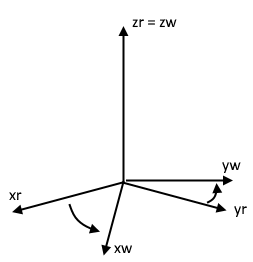
\includegraphics[width=2in]{figures/coordrobottoworld.png}
  \caption[Coordinates from robot to world] {Rotation and translation from Robot to World}
  \label{fig:coordrobottoworld}
\end{figure}

The following equation:
\begin{align*}
\begin{bmatrix}
x_r \\
y_r \\
1 
\end{bmatrix}
= \underbrace{\begin{bmatrix}
a & b & c \\
d & e & f \\
g & h & i 
\end{bmatrix}}_{\text{}}
\begin{bmatrix}
x_w \\
y_w \\
1 
\end{bmatrix}
\end{align*}
%Its just to maintain the order. 
%
%figure
%one frame here and one frame here... Do the rotation here...
%
%Then we can find this equations...
%
%Translation matrix and rotation matrix... Now we have 9 unknowns we need 9 equations...
\begin{align}
Trans_{mat} = experimentalTrans();
\end{align}

To calculate the hej matrix it is need to have 9 equations since we have 9 unknows. To create these 9 different equations we need 3 different coordinates in the robot and the world frame. The reason for 3 different coordinates is because every coordinate has both a x,y and z value. These coordinates is achieved by putting the robot manually at 3 different points and measuring the coordinate in the robot and world frame. The 9 different equations will then be:
\begin{align*} 
x_r(p_1) &= a\cdot x_w(p_1) + b\cdot y_w(p_1) + c \\
y_r(p_1) &= d\cdot x_w(p_1) + e\cdot y_w(p_1) + f \\
1 &= g\cdot x_w(p_1) + h\cdot y_w(p_1) + k \\
x_r(p_2) &= a\cdot x_w(p_2) + b\cdot y_w(p_2) + c\\
y_r(p_2) &= d\cdot x_w(p_2) + e\cdot y_w(p_2) + f \\
1 &= g\cdot x_w(p_2) + h\cdot y_w(p_2) + k \\
x_r(p_3) &= a\cdot x_w(p_3) + b\cdot y_w(p_3) + c \\
y_r(p_3) &= d\cdot x_w(p_3) + e\cdot y_w(p_3) + f \\
1 &= g\cdot x_w(p_3) + h\cdot y_w(p_3) + k
\end{align*}
And the points:
Experimental Transformation matrix. The code is in appendix \ref{app:experimentaltrans}
\begin{align*}
x1_w&=28*[-1\quad -1] x2_w&=28*[-1\quad 6]  x3_w&=28*[5\quad 2]\\
x1_r&=[239.484\quad 198.714] x2_r&=[233.953\quad 398.995]   x3_r&=[408.578\quad 287.651]
\end{align*}
Calculations using the origin to get the w (last value of the matrix Values)
Origin
\begin{lstlisting}

img_og = Proj*[0;0;1];
w_og = img_og(3);
img_og = img_og/w_og;
\end{lstlisting}
Corners
\begin{lstlisting}
img_cur = Proj*[29*8;0;1];
w_cur = img_cur(3);
img_cur = img_cur/img_cur(3);
img_cul = Proj*[29*8;29*5;1];
w_cul = img_cul(3);
img_cul = img_cul/img_cul(3);
img_cdl = Proj*[0;29*5;1];
w_cdl = img_cdl(3);
img_cdl = img_cdl/img_cdl(3);
\end{lstlisting}
W term
\begin{lstlisting}
w = [w_og; w_cur; w_cul; w_cdl];
% fprintf('Deviation (w): %f\n',w);
\end{lstlisting}




















%We need to use the checkerboard. We knew that this 0 was the origin and then choose 3 different points. 
%From the gripper we found the robot coordinates and read from the screen...
%
%Then we solved the 9 equations and used 3 different points and we got the 9 equations and solved it... 
%
%We had the world coordinate and we needed the robot. And this was something that was difficult to do. And easy to do with 9 equations. We needed to give the value to the robot to tell it to go the specific position. We needed to build some relationship between the world and the robot and as you can see in this frame you have this coordinate and in this frame you have this coordiante. 
%
%By doing this we can find the transformation from the world to the robot.
%
%extrinsic
%\begin{align}
%\text{extrinsic} = 
%\begin{bmatrix}
%    \text{Rc\_ext} & \text{Tc\_ext} 
%\end{bmatrix}
%\end{align}
%Extrinsic and Intrinsic Matrices are used to change the coordinate systems
%Intrinsic
%\begin{align}
%\text{KK} &= 
%\begin{bmatrix}
%    1666.6 & 0 & 1153.2 \\
%    0 & 1666.2 & 750.4 \\
%    0 & 0 & 1 
%\end{bmatrix} \\
%\text{intrinsic} &= \text{KK}
%\end{align}
%Projection
%\begin{align}
%\text{Proj} = \text{intrinsic}*\text{extrinsic}; 
%\end{align}
%We can ignore the third column because the Z coordinate is always zero. So we will have a 3x3 matrix and we will be able to inverse it.
%\begin{align}
%\text{Proj(:,3)}=[];
%\end{align}
%World - Robot Transformation Matrix
%\begin{align}
%\text{Trans\_mat} = 
%\begin{bmatrix}
%    cos(\theta_r) & -sin(\theta_r) & 0 & 266.672 \\
%    sin(\theta_r)  & cos(\theta_r) & 0 & 226.186 \\
%        0         &      0         & 1 &    0 
%\end{bmatrix}
%\end{align}
%
